%!TEX root = main.tex
\chapter[Evaluaci\'on]{Evaluaci\'on}
\label{cap:evaluation}

En la secci\'on \ref{sec:intro.objetivos} definimos las motivaciones y objetivos de esta tesis, donde el principal consta del dise\~no y desarrollo de un operador de mutaci\'on, altamente configurable, para expresiones encadenadas. Luego, en la secci\'on \ref{sec:preliminares.mutation.opevaluation} definimos que propiedades afectan el an\'alisis de \emph{mutation testing}, cantidad de mutantes, mutantes equivalentes, dificultad de detecci\'on, acoplamiento con fallas reales, y redundancia de mutantes (o acoplamiento entre mutantes). En este capitulo realizamos la evaluaci\'on de nuestro ``meta-operador'', \emph{prvo}, para determinar la utilidad pr\'actica de la misma.

\section{Configuraci\'on}
\label{sec:evaluation.prvoconfig}

Antes de evaluar a \emph{prvo}, es necesario que definamos una configuraci\'on particular para el mismo. Teniendo en cuenta que la configuraci\'on sobre miembros de clases a utilizar o evitar, es decir, una de las propiedades principales que regula el conjunto de expresiones a utilizar durante la mutaci\'on, es algo que debe definirse por cada proyecto, vamos entonces para este caso, a definir de manera general que criterio vamos a utilizar para configurar esta propiedad para cada proyecto. El primer problema a resolver para poder definir esta configuraci\'on y el criterio para expresiones a utilizar, es especificar que tipo de fallas estamos interesados en representar, puesto que lo mejor no es una configuraci\'on que permita representar m\'ultiples fallas sino una que se centre en un tipo de falla espec\'ifica. De acuerdo a nuestro ejemplo motivador, dado en la secci\'on \ref{sec:intro.objetivos}, el tipo de fallas que queremos representar son aquellas que involucran expresiones de navegaci\'on, es decir, expresiones encadenadas de tama\~no al menos 1, y que resultan de el acceso al miembro incorrecto de una clase. Estas fallas no parecen estar de acuerdo con el ejemplo, recordemos que \'este utiliza un m\'etodo \emph{dequeue()} que solo tiene una l\'inea donde reasigna el valor a un puntero, y la falla est\'a en la falta de c\'odigo, como controles y reasignaci\'on de otros punteros, sin embargo, modificar un miembro en las expresiones halladas en la \'unica sentencia del m\'etodo, genera la necesidad de mejorar el test suite. Por parte de las fallas mencionadas como no acopladas actualmente a fallas reales, descriptas en \ref{sec:prvo.prvoTargetedFaults}, dentro de estas vamos a estar representando a:

\begin{enumerate}[label=\arabic*), leftmargin=.75cm,align=left]
	\item Llamada a un m\'etodo similar de la misma librer\'ia
	\item Acceso directo a un campo\footnote{Solo para campos de las clases bajo evaluaci\'on}
\end{enumerate}

\'Esto parecer\'ia un objetivo bastante peque\~no con respecto a las fallas a representar, pero todo el desarrollo e investigaci\'on que rodea a \emph{prvo} siempre puso en evidencia cuan f\'acil es que una configuraci\'on poco restrictiva, lleve a una explosi\'on en la cantidad de mutantes generados, no solo \'esto, la cantidad de mutantes irrelevantes generados constitu\'ia un gran porcentaje de los mismos. [NUMEROS DE MUTANTES GENERADOS EN STRYKER PODRIA SERVIR ACA]

Pasemos entonces a definir la configuraci\'on a utilizar:

\subsubsection{Expresiones objetivo}

Las expresiones que vamos a mutar son aquellas que sean expresiones de navegaci\'on y se encuentren en cualquier contexto, asignaciones (parte izquierda y derecha), expresiones unarias y binarias, sentencias de retorno, ciclos y llamadas a m\'etodos, etc.

\subsubsection{Expresiones a utilizar}

Con respecto a las expresiones que se van a utilizar al mutar una expresi\'on, se va a restringir el uso a solo aquellas que pertenezcan a la clase principal bajo evaluaci\'on o aquellas relacionadas a la estructura principal que \'esta representa, recordemos que nuestros casos de estudio van a estar compuestos por estructuras de datos. Ejemplo de \'esto es, para la clase \emph{LinkedList} solo se van a poder utilizar miembros de la misma y de la clase \emph{Node} utilizada por \'esta. Es necesario aclarar que las variables alcanzables tambi\'en van a ser consideradas.

El control de tipos va a ser estricto, lo que significa que una subexpresi\'on solo puede intercambiarse por otra con \textbf{exactamente} el mismo tipo. Al tener como objetivo a expresiones de navegaci\'on, el uso de literales no tiene mucho sentido, \'esto no significa no utilizar constantes como por ejemplo definir el puntero al comienzo de la lista con \emph{final}, o definir un nodo ficticio de nuevo con el mismo modificador. El uso de campos est\'aticos solo se va a permitir dentro de un contexto est\'atico, por ejemplo, en el m\'etodo \lstinline|public static int foo()|, se van a permitir miembros est\'aticos, pero en el m\'etodo \lstinline|public int bar()|, no.

\section{Operadores a utilizar}
\label{sec:evaluation.operators}

Para nuestros experimentos vamos a seleccionar todos los operadores b\'asicos, que aplican a nivel de m\'etodo, implementados en \emph{$\mu$Java++}. \'Estos son un conjunto que incluye al conjunto de operadores suficientes definidos en \ref{sec:preliminares.mutation.sufficient}, excepto por \emph{ABS} (el cual cambia expresiones aritm\'eticas a 0, un valor positivo, y un valor negativo) por no estar implementado en \emph{$\mu$Java} y por lo tanto no lo est\'a en \emph{$\mu$Java++}.

\begin{description}[leftmargin=8em,style=nextline]
	\item[AODS] Elimina los operadores aritm\'eticos de incremento y decremento (pre-decremento: \emph{--exp}; pre-incremento: \emph{++exp}; pos-decremento: \emph{exp--}; y pos-incremento: \emph{exp++}).
	\item[AODU] Elimina los operadores aritm\'eticos unarios (\emph{+exp} y \emph{-exp}).
	\item[AOIS] Inserta los operadores aritm\'eticos de incremento y decremento en variables y campos de clases.
	\item[AOIU] Inserta los operadores aritm\'eticos unarios en expresiones artim\'eticas.
	\item[AORB] Reemplaza operadores aritm\'eticos binarios por otros, en una expresi\'on binaria.
	\item[AORS] Reemplaza operadores aritm\'eticos de incremento y decremento.
	\item[AORU] Reemplaza operadores aritm\'eticos unarios en expresiones.
	\item[ASRS] Reemplaza los operadores de asignaci\'on compuestos por otros del mismo tipo, \'estos operadores de asignaci\'on, permiten reemplazar expresiones del tipo \textbf{x = x op y} por \textbf{x op= y}, por ejemplo \textbf{x += y}.
	\item[COD] Elimina el operador unario de negaci\'on condicional.
	\item[COI] Inserta el operador unario de negaci\'on condicional a expresiones de tipo booleano.
	\item[COR] Reemplaza operadores condicionales binarios por otros (\emph{\&\&}, \emph{||}). Si bien no considerados condicionales, los operadores l\'ogicos pueden ser utilizados tambi\'en por este operador, incluyendo el ``y'' (\emph{\&}), ``o'' (\emph{|}), y ``xor'' (\emph{\^}) bit a bit.
	\item[LOD] Elimina el operador l\'ogico de negaci\'on binaria (\emph{~}).
	\item[LOI] Inserta el operador l\'ogico de negaci\'on binaria.
	\item[LOR] Reemplaza operadores l\'ogicos binarios por otros (\emph{\&}, \emph{|}, \emph{\^}).
	\item[ROR] Reemplaza operadores relacionales con otros (\emph{<}, \emph{<=}, \emph{>}, y \emph{>=}), y reemplaza todo un predicado por \emph{verdadero} y \emph{falso}.
\end{description}

\section{Evaluaci\'on}
\label{sec:evaluation.evaluation}

El objetivo de la evaluaci\'on es analizar si \emph{prvo}, como familia de operadores de mutaci\'on para expresiones encadenadas, es de hecho una contribuci\'on a \emph{mutation testing}. La contribuci\'on te\'orica de nuestra familia de operadores queda clara en nuestras motivaciones y el dise\~no de \emph{prvo}:
\begin{quote}
  Existen fallas reales relacionadas a expresiones encadenadas que no son representadas por mutantes generados por operadores de mutaci\'on existentes.
\end{quote}
Sin embargo, la contribuci\'on en la pr\'actica puede no existir, \emph{las fallas que representa prvo est\'an subsumidas por aquellas que representan operadores existentes}; \emph{las mutaciones generadas por prvo son triviales de detectar, o son equivalentes}; \emph{la cantidad de mutantes generados por prvo excede los potenciales beneficios de su uso}. Es por esto que nuestra evaluaci\'on se centra en las siguientes preguntas:
\begin{itemize}
	\item \textbf{RQ1} El uso de \emph{prvo} complementa de manera significativa a los operadores de mutaci\'on tradicionales?
	
	\item \textbf{RQ2} Cual es el costo adicional de utilizar \emph{prvo}, en mutation testing?
\end{itemize}

La motivaci\'on para \textbf{RQ1} est\'a basada en que un nuevo operadores no ser\'ia \'util si fuera redundante con respecto a los existentes. Para responder \textbf{RQ1} vamos a utilizar \emph{dynamic mutant subsumption}. Este an\'alisis permite, para un programa particular y un conjunto de tests particulares, evaluar que mutantes resultan indispensables y cuales son redundantes para la evaluaci\'on del conjunto de tests. Vamos a utilizar principalmente como benchmark, implementaciones de estructuras de datos orientadas a objetos, en \emph{Java}. La raz\'on para considerar un benchmark as\'i, es que este tipo de implementaciones hace un uso substancial de expresiones de navegaci\'on, incluyendo tipos recursivos de datos. Nuestro benchmark va a estar compuesto entonces mayormente por implementaciones de collecciones:  \emph{Apache's TreeList}, una implementaci\'on de listas utilizando \'arboles; \emph{Apache's NodeCachingList}, una lista encadenada con una cach\'e de nodos; \emph{AvlTree}, una implementaci\'on cl\'asica de \'arboles balanceados; \emph{BinomialHeap}, una implementaci\'on basada en referencias de mont\'iculos; y \emph{TreeSet}, una implementaci\'on de conjuntos utilizando \'arboles red-black. %TODO: AGREGAR CASOS

Para responder a \textbf{RQ1} vamos a utilizar mutation score, toughness (cuantos tests un mutante sobrevive antes de ser detectado), y dynamic mutant subsumption para detectar mutantes dominadores. Adem\'as se van a analizar los mutantes no detectados para detectar aquellos que son equivalentes, esto solo se va a realizar para aquellos generados por \emph{prvo}. A su vez, si bien en principio evaluar cuantos nodos dominadores involucran a \emph{prvo} parece una buena m\'edida, es importante destacar que un nodo puede contener varios mutantes equivalentes entre s\'i, entonces utilizar directamente la relaci\'on \texttt{(nodos dominadores que involucran a prvo)/total de nodos dominadores}, no sirve de mucho por que la informaci\'on obtenida no va a necesariamente reflejar cuanto domina \emph{prvo} sobre todos los mutantes. Por esto, vamos a utilizar el concepto de nodos puros descripto previamente en \ref{sec:implementation.dynamicSubsumption.graph} para poder medir la relaci\'on de nodos puros dominadores de \emph{prvo}.

Vamos a necesitar proveer conjuntos de tests para realizar nuestra evaluaci\'on. Sobre todo, para que nuestro an\'alisis sea significativo, necesitar\'iamos utilizar conjuntos de tests relativamente ``buenos'', dado que si fu\'eramos a utilizar test suites pobres (con baja cobertura de c\'odigo por ejemplo), podr\'iamos no obtener relaciones entre el uso o no de \emph{prvo}, o resultados que solo se mantienen al usar tests de mala calidad.

Dynamic mutant subsumption es un an\'alisis que se ve beneficiado por tener gran cantidad de tests. Entonces es necesario establecer como vamos a generar nuestros tests. Manualmente, tiene la ventaja de hacer tests teniendo un conocimiento de no solo la sem\'antica del programa bajo prueba, sin\'o un tambi\'en de la sint\'axis. Las desventajas vienen por dos lados, por uno, generar manualmente una gran cantidad de tests, representa un trabajo complejo y tedioso; por el otro lado, no es posible garantizar imparcialidad, incluso de manera subconsciente uno podr\'ia caer en la tentaci\'on de escribir tests sabiendo el impacto que los mismos van a tener en la evaluaci\'on de \emph{prvo}. Autom\'aticamente, tiene la ventaja de que permite generar una gran cantidad de tests, tan grande como uno quiera para algunas herramientas, y brinda imparcialidad. Al mismo tiempo, utilizar herramientas autom\'aticas permite generar varios test suites distintos con la misma ``calidad'', lo cual nos sirve para poder repetir los experimentos y eliminar, al menos en cierto grado, la incertidumbre de si nuestros resultados son buenos por que usamos un conjunto de tests particularmente favorable para nosotros. 

Dentro de las herramientas de generaci\'on autom\'atica de tests, creemos que \emph{Evosuite} y \emph{Randoop} son dos de las mejores en la actualidad, al menos para \emph{Java}. Evosuite utiliza algor\'itmos gen\'eticos para, a partir de un conjunto inicial de test suites, hacer evolucionar a estos hasta lograr el ``mejor''. Si bien Evosuite suele generar buenos tests, el inconveniente para nuestro estudio es que \'estos son relativamente pocos, incluso si se incrementan los recursos disponibles para la herramienta, lo \'unico que se mejora son la calidad de los tests generados (con respecto a uno o varios criterios de evaluaci\'on), pero como dijimos, necesitamos conjuntos grandes de tests. Es por esto que creemos que complementar los tests de Evosuite con los generados por Randoop, una herramienta que genera tests mediante aleatoriedad en donde la cantidad de tests generados se puede controlar con los recursos utilizados, es la mejor forma para generar los test suites que vamos a utilizar para evaluar \emph{prvo}.

Nuestro an\'alisis tienen que tener en cuenta a \emph{prvo} como un operador adicional\footnote{La familia de operadores de \emph{prvo} la consideremos como un solo operador.}. Los otros operadores de mutaci\'on, con los que vamos a comparar, son aquellos considerados en el conjunto de operadores de mutaci\'on suficientes \cite{bibliography.mutation.selection.Offutt96, bibliography.mutation.selection.ASN2008} e implementados en \emph{mu$Java$}. Detalles de todos los operadores a nivel de m\'etodo soportados por \emph{mu$Java$} y subsecuentemente por \emph{mu$Java$++} pueden encontrarse en \cite{muJavaMOPS}. 

Si bien cuando mencionamos las propiedades a tener en cuenta en el dise\~no de operadores de mutaci\'on, vimos que la mayor\'ia de las mismas tienen un gran impacto en el significado del mutation score obtenido, \'este sigue siendo un valor com\'unmente utilizado en estudios, y representa \textbf{el} indicador asociado a \emph{mutation testing}. Por lo tanto nos interesa observar como \'este es afectado por la inclusi\'on de \emph{prvo}. Teniendo en cuenta que, una suba en el mismo representar\'ia el hecho de que \emph{prvo} gener\'o mutantes que en su mayor\'ia fueron detectados; mientras que una baja, representar\'ia que \emph{prvo} gener\'o mutantes que representan nuevas fallas no detectadas por el test suite. Es necesario aclarar, que en cualquier caso, no es posible sacar conclusiones solamente basados en estos cambios, por eso analizamos equivalencia y dominancia.

Tal como describimos en la secci\'on \ref{sec:implementation.dynamicSubsumption.graph}, nuestro an\'alis va a utilizar informaci\'on obtenida de los grafos de \emph{dynamic mutant subsumption}, particularmente como cambia la representaci\'on de los operadores en los nodos dominantes, con y sin \emph{prvo}. La pureza de los nodos nos va a ser de gran utilidad en este an\'alis para poder eliminar los casos en donde mutantes generados por distintos operadores tienen gran presencia en los nodos dominantes, pero son equivalentes entre s\'i.

Para poder evitar casos donde el test suite utilizado es particularmente beneficioso o desfavorable para \emph{prvo}, vamos a realizar m\'ultiples experimentos para el mismo programa con distintos test suites generados de manera autom\'atica. Dado que las herramientas utilizadas tienen ambas distintos grados de aleatoriedad, vamos a utilizar un conjunto fijo de ``semillas'' para garantizar cierto grado de replicaci\'on. Incluso con la misma semilla, al ser herramientas que se ejecutan con un presupuesto de tiempo determinado, la cantidad de operaciones que logran realizar bajo \'este, no siempre es la misma, generando no determinismo. Creemos que la repetici\'on de nuestros experimentos es suficiente para contrarrestar los efectos del mismo.

Respecto a \textbf{RQ2}, el foco est\'a en la eficiencia; incluso si \emph{prvo} (o cualquier operador) resulta ser \'util en cuanto a los mutantes que genera, su uso se vuelve prohibitivo si los costos asociados a su utilizaci\'on son muy altos. Este costo est\'a t\'ipicamente asociado a dos factores: la complejidad en la generaci\'on de los mutantes, y el n\'umero de mutantes generados. El primero es com\'unmente ignorada, dado que salvo casos muy raro, los recursos utilizados son usualmente despreciables. El segundo factor es en general el que representa la preocupaci\'on principal para el dise\~no de un operador de mutaci\'on, dado que en el peor caso, todos los tests deben ser ejecutados para todos los mutantes al computar el \emph{mutation score}. Es por eso que cuantos mutantes genera \emph{prvo} es la m\'etrica principal para analizar su costo.

%Due to space restrictions, we only report here a summary of the experimental results. Further information, along with a replication package, can be found in:
%\begin{center}
%	\texttt{https://sites.google.com/view/prvo/}
%\end{center}

\section{Resultados experimentales}
\label{sec:evaluation.results}

En esta secci\'on vamos a discutir los resultados de nuestra evaluaci\'on, enfoc\'andonos primero en \textbf{RQ1}. La figura \ref{subsumption-results} resume los resultados de nuestro an\'alisis de subsuma. Los resultados se muestran por caso de estudio. Cada gr\'afico incluye el porcentaje de mutantes dominantes por operador de mutaci\'on, usando la media de todas las repeticiones para el mismo caso de estudio. \'Estas representan los experimentos, que como anteriormente explicado, incluyen una ejecuci\'on usando \emph{prvo} junto a los operadores descriptos en \ref{sec:evaluation.operators}, y otra donde solo \'estos fueron utilizados.

Los resultados para los experimentos que no utilizan \emph{prvo} se muestran con barras verdes. Por ejemplo, para \emph{TreeList}, los mutantes generados por el operador \emph{LOI} (el cual inserta el operador de complemento binario \emph{~}) representan un poco m\'as del 35\% de los mutantes dominadores, cuando \emph{prvo} no es utilizado. Al tener en cuenta \emph{prvo}, y ejecutar nuevamente los experimentos, estos porcentajes cambian. Los resultados correspondientes a los experimentos donde el operador \emph{prvo} es utilizado, se muestran en barras rojas. Por ejemplo, para el mismo caso anterior (TreeList), el porcentaje de mutantes dominadores \emph{LOI} disminuyen a menos del 30\%. En este mismo caso, los mutantes dominadores de \emph{prvo} representan un 25\% de todos los dominadores.

Es necesario resaltar en los resultados mostrados en las tablas de la Figura-\ref{subsumption-results}, el valor correspondiente a \emph{dominadores puros}. Como se describi\'o en \ref{sec:implementation.dynamicSubsumption.graph}, al construir el grafo de subsuma de mutantes, aquellos mutantes que son equivalentes entre s\'i, es decir, se subsuman el uno al otro, se encapsulan en el mismo nodo del grafo. \'Esto, lleva a que si un nodo es considerado dominador (no es subsumido por ning\'un otro nodo, o, lo que es lo mismo a que no existen arcos que partan de otro nodo hacia \'este) todos los mutantes dentro del nodo son, a su vez, considerados dominadores. La existencia de nodos dominadores constitu\'idos por mutantes que fueron generados por otros operadores, afecta de manera negativa a nuestras conclusiones, podr\'iamos decir que \emph{prvo} domina cuando en realidad existen mutantes de otros operadores que son equivalentes, con respecto a \emph{dynamic mutant subsumption}. Es por esto que introdujimos el concepto de \emph{dominadores puros}, para poder evaluar cuando mutantes de un operador dominan sin ser equivalentes a otros. Esta informaci\'on se muestra con barras azules. Por ejemplo, para \emph{TreeList}, m\'as del 20\% de los mutantes dominadores de \emph{prvo} son considerados puros.

La observaci\'on m\'as importante al analizar los resultados es que, en casi todos los casos (con la excepci\'on de \emph{NodeCachingList}), \emph{prvo} se posiciona entre los mejores, con respecto a dominancia, incluso es uno de los mejores tres operadores dominantes, junto a operadores t\'ipicos del conjunto de \emph{suficientes}, como \emph{ROR}, \emph{LOI}, y la familia de operadores de mutaci\'on que corresponden a la inserci\'on de operadores aritm\'eticos (\emph{AOIS}, \emph{AOIU}, y \emph{AOIB}). Es tambi\'en importante de remarcar que, en presencia de \emph{prvo}, la dominancia de otros operadores es en general reducida, y su dominancia sobre ciertos nodos es ``transferida'' hacia \emph{prvo}. M\'as precisamente, \emph{prvo} domina sobre ciertos mutantes previamente (en ausencia de \emph{prvo}) dominantes.

Claramente, nuestros resultados experimentales resultan en una respuesta positiva a \textbf{RQ1}: \emph{prvo} complementa de manera significativa al conjunto de operadores tradicionales; los mutantes producidos son en general no dominados por operadores existentes, y exhibe un alto n\'umero de mutantes dominantes, lo que nos permitir\'ia considerar, al menos en el contexto de nuestros experimentos, a \emph{prvo} como un operador ``suficiente'', junto al conjunto de operadores suficientes tradicionales.

\begin{figure}[t]
	\begin{center}
		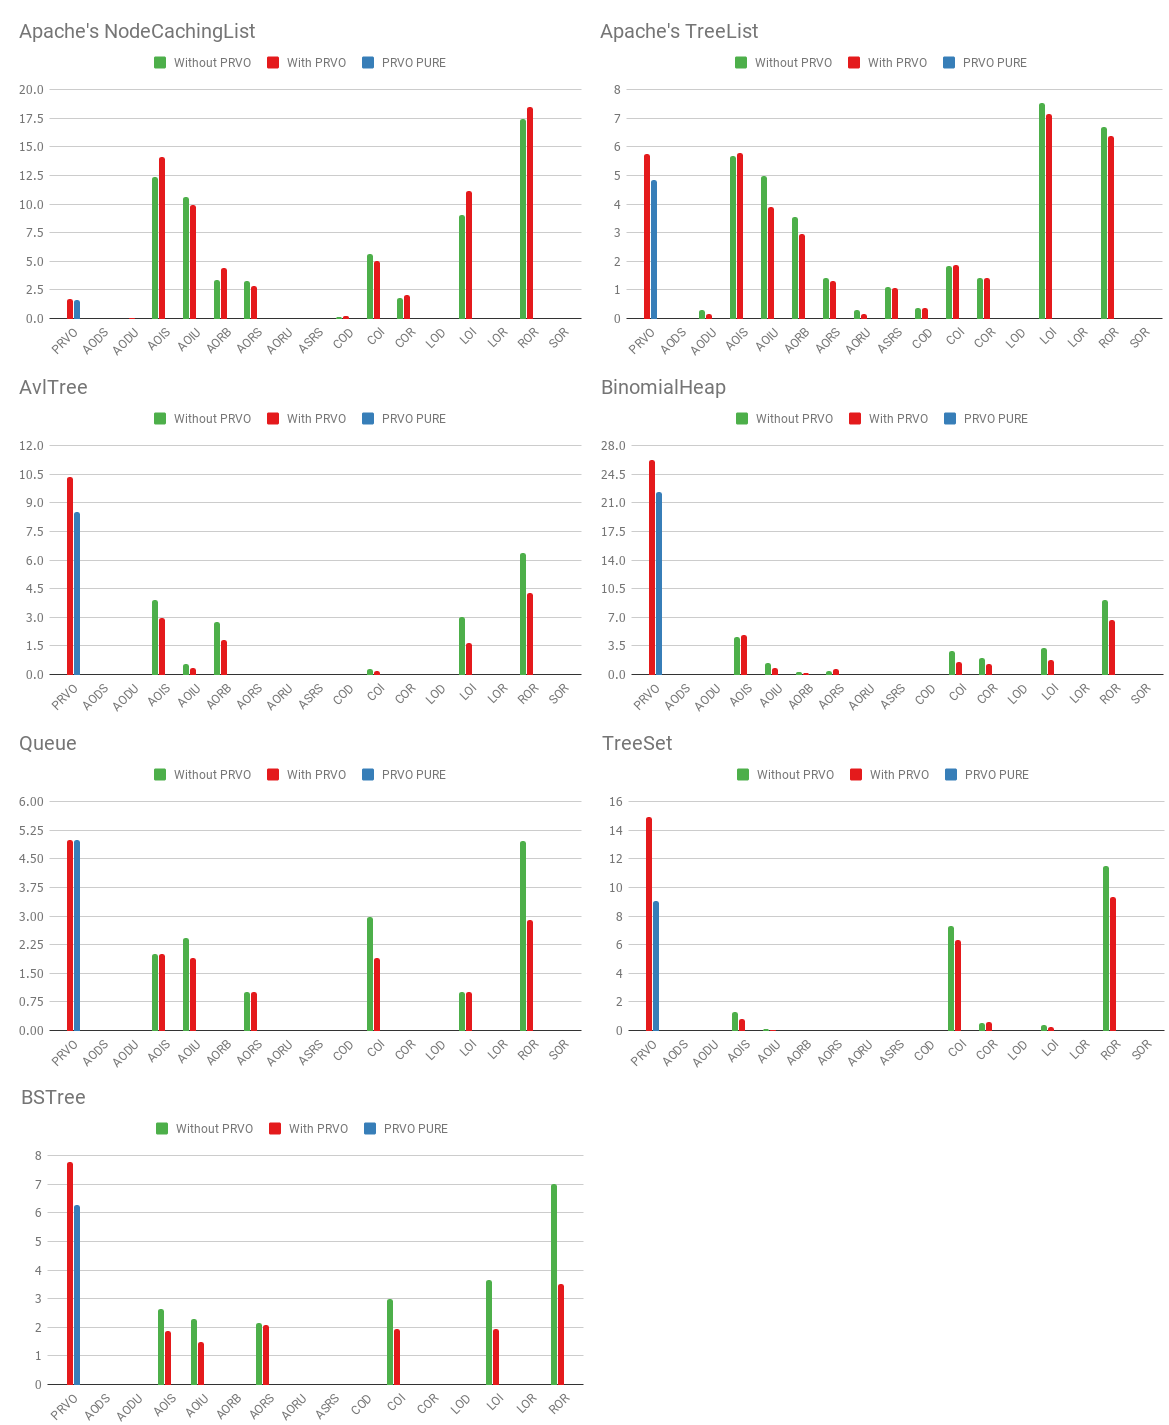
\includegraphics[width=12cm]{figures/Tables.png}
	\end{center}
	\caption{Summary of dynamic subsumption analysis}
	\label{subsumption-results}
\end{figure}

Analicemos ahora \textbf{RQ2}. La Figura-\ref{mutants-results} resume los resultados para generaci\'on de mutantes, comparando el n\'umero de mutantes obtenidos cuando \emph{prvo} no es inclu\'ido (barras verdes), con los casos en donde \emph{prvo} es considerado (barras azules). Reportamos tambi\'en, en estas tablas, el n\'umero de mutantes equivalentes de \emph{prvo} (mutantes que son sem\'anticamente equivalentes al programa original, y por lo tanto imposibles de detectar con cualquier test) producidos para cada caso de estudio.

Para la mayor\'ia de los casos de estudio, el n\'umero de mutantes que genera \emph{prvo} representa solo un peque\~no incremento sobre la cantidad de mutantes generados por los operadores tradicionales. Los casos de estudio \emph{TreeSet} y \emph{BinomialHeap} son dos excepciones, en donde la cantidad de mutantes generados por \emph{prvo} representa pr\'acticamente la misma que la generada por todos los operadores tradicionales por si solos. La raz\'on es que estos casos de estudios se caracterizan por una gran cantidad de m\'etodos conteniendo, a su vez, una gran cantidad de expresiones de navegaci\'on en condiciones y otras comparaciones, del tipo \texttt{expr == null}. Estas expresiones admiten una sola mutaci\'on de parte de \emph{ROR} (reemplazar el igual por un distinto), pero en donde \emph{prvo} produce muchas mutaciones. Sin embargo, en estos dos estudios, hay que notar que \emph{prvo} es claramente dominante (como se ve en la Figura-\ref{subsumption-results}); en particular, es notable como la dominancia de otros operadores es disminu\'ida significativamente cuando \emph{prvo} es utilizado. Nuestra respuesta entonces para \textbf{RQ2}, es que el costo adicional, con respecto a cantidad de mutantes, de utilizar \emph{prvo}, es en general bajo, aunque existen casos en donde el n\'umero de mutaciones generadas por \emph{prvo} puede ``explotar''. Estos casos muestran, en nuestros experimentos, una gran dominancia por parte de \emph{prvo} sobre mutaciones producidas por otros operadores, sugiriendo que existe un margen para realizar optimizaciones mediante priorizaci\'on de tests/mutantes, una t\'ecnica que consiste en ordenar y/o seleccionar tests o mutantes para ser evaluados antes que otros, o en lugar de otros, as\'i disminuir los recursos necesarios. De todas formas, estos resultados sugieren realizar refinamientos a \emph{prvo}, ya sea a\~nadiendo an\'alisis durante la generaci\'on de mutaciones, o implementando nuevas propiedades para configurar a \emph{prvo} de manera m\'as apropiada para cada caso. \'Esto, puede llevar a lograr una mejor eficiencia, es decir una menor cantidad de mutantes, por parte de \emph{prvo}.

Con respecto a mutantes equivalentes, los resultados son muy interesantes. La cantidad de mutantes equivalentes producidos por \emph{prvo} fue muy poca. \'Esto, es muy importante, dado que cuando un operador produce muchos mutantes equivalentes, es decir, mutantes para los cuales no existe ning\'un escenario o entrada para el cual \'este se comporte de manera diferente al programa original, lo que lo hace imposible de detectar, bajando el valor de mutation score correspondiente de manera artificial, resultando en una evaluaci\'on enga\~nosa del test suite. Tener entonces una peque\~na cantidad de dichos mutantes es un buen resultado para \emph{prvo}. Vale la pena aclarar que si bien lo deseable es evitar por completo la generaci\'on de mutantes equivalentes, \'esto es en general imposible, principalmente por que al ser un problema indecidible (el detectar si un programa es equivalente a otro), no es posible tener una implementaci\'on de una herramienta de mutaci\'on que evite por completo la generaci\'on de los mismos.

\begin{figure}[t]
	\begin{center}
		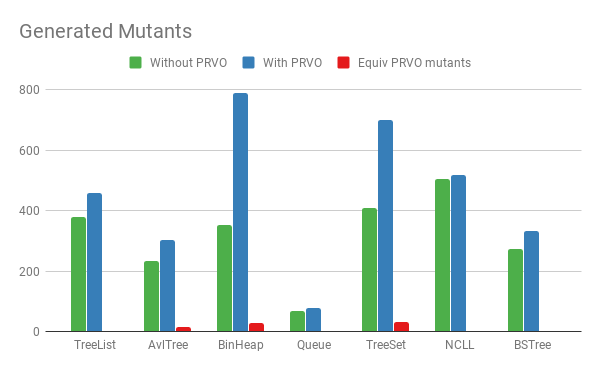
\includegraphics[width=9cm]{figures/Generated_Mutants.png}
	\end{center}
	\caption{Summary of mutants generated.}
	\label{mutants-results}
\end{figure}


\section{Amenazas a la validez}

Nuestra evaluaci\'on experimental est\'a limitada a implementaciones relativamente peque\~nas de colecciones en \emph{Java}. Las razones por las que seleccionamos estas implementaciones como casos de estudio fueron parcialmente descriptas anteriormente, y esencialmente tiene que ver con que estos proyectos son buenos representantes de implementaciones orientadas a objetos con usos sofisticados de expresiones de navegaci\'on (por ejemplo, utilizan tipos de datos recursivos, y m\'ultiples referencias a objetos distintos del mismo tipo). Otra raz\'on por la que nos limitamos a estos casos de estudio tiene que ver con el alto costo de an\'alisis de mutaci\'on. Especialmente en nuestro contexto, en donde las caracter\'isticas de nuestra evaluaci\'on nos lleva a la necesidad de realizar numerosos an\'alisis de mutaci\'on, en particular, computar los grafos de subsuma de mutantes har\'ia inviable esta evaluaci\'on si fu\'eramos a utilizar proyectos m\'as grandes.

Nuestro an\'alisis est\'a tambi\'en atado a una forma espec\'ifica de generar tests, \'esta se basa en el uso de dos herramientas particulares, Evosuite y Randoop espec\'ificamente. \'Esto est\'a motivado por el tipo de test suites que resultan de relevancia para an\'alisis de subsuma. Dado el impacto que tiene el presupuesto de tiempo que se brinda a las herramientas que utilizamos para generar los test suites, nuestros resultados podr\'ian estar siendo afectados por el mismo. Para contrarrestar esta potencial amenaza, corrimos los experimentos con distintos presupuestos de tiempo, lo que llev\'o a test suites de distintos tama\~nos, y por supuesto resultados diferentes. Sin embargo \'estos son consistentes, es decir, las observaciones para un experimento mantienen la misma tendencia para todos los presupuestos de tiempo utilizados.

Gran parte de nuestra evaluaci\'on experimental es m\'as bien objetiva, por ejemplo, la noci\'on de subsuma, y est\'an calculadas por nuestra implementaci\'on. Hicimos nuestro mejor esfuerzo para garantizar la validez de nuestros resultados, pero a\'un as\'i nuestra implementaci\'on podr\'ia contener defectos que afecten a nuestros resultados. La equivalencia de programas, requerida para analizar mutantes equivalentes, es un problema indecidible. Varias t\'ecnicas han sido propuestas para resolver este problema (obviamente de manera aproximada), sin embargo, la verificaci\'on manual sigue siendo una de las m\'as utilizada en la pr\'actica, y es la que hemos utilizados nosotros. Afortunadamente este an\'alisis estuvo limitado a un n\'umero muy peque\~no de mutantes y cualquier duda sobre la equivalencia de uno, fue siempre anotada en desventaja de \emph{prvo}, es decir, ante la duda, se consider\'o el mutante como equivalente. Creemos que los errores que podemos haber cometido con respecto a equivalencia de mutantes, no afectan de manera significativa nuestras conclusiones.

Nuestro an\'alisis est\'a tambi\'en limitado a un conjunto arbitrario de operadores de mutaci\'on. Podr\'iamos haber considerado otros operadores, por ejemplo los que act\'uan a nivel de clases (en contraposici\'on de los que usamos que act\'uan a nivel de m\'etodos) \cite{bibliography.mutation.class-level-ops}. \'Estos, est\'an relacionados a nuestro trabajo, en el sentido de que se aplican a programas orientados a objetos, pero se enfocan en aspectos ortogonales como visibilidad (cambiando la visibilidad de m\'etodos y campos en una clase). Decidimos concentrarnos en los operadores que se consideran tradicionales, en el contexto de mutation testing, y creemos que hemos tenido en cuenta a los m\'as significativos, basado en los que est\'an disponibles en las herramientas de mutation testing, y en estudios de operadores suficientes.

Finalmente necesitamos remarcar que subsuma de operadores, no es lo mismo que subsuma de mutantes. El primero es una relaci\'on entre operadores que es independiente de que programa se est\'e mutando, se trata de una relaci\'on que o bien se explica por la misma definici\'on de los operadores, o bien (como sucede en la mayor\'ia de los casos) requiere numerosos experimentos para determinar si es posible concluir si un operador subsume a otro. Sin embargo nuestra evaluaci\'on de subsuma din\'amica de mutantes, permite, de manera indirecta, una evaluaci\'on de la primera.